\documentclass[1p]{elsarticle_modified}
%\bibliographystyle{elsarticle-num}

%\usepackage[colorlinks]{hyperref}
%\usepackage{abbrmath_seonhwa} %\Abb, \Ascr, \Acal ,\Abf, \Afrak
\usepackage{amsfonts}
\usepackage{amssymb}
\usepackage{amsmath}
\usepackage{amsthm}
\usepackage{scalefnt}
\usepackage{amsbsy}
\usepackage{kotex}
\usepackage{caption}
\usepackage{subfig}
\usepackage{color}
\usepackage{graphicx}
\usepackage{xcolor} %% white, black, red, green, blue, cyan, magenta, yellow
\usepackage{float}
\usepackage{setspace}
\usepackage{hyperref}

\usepackage{tikz}
\usetikzlibrary{arrows}

\usepackage{multirow}
\usepackage{array} % fixed length table
\usepackage{hhline}

%%%%%%%%%%%%%%%%%%%%%
\makeatletter
\renewcommand*\env@matrix[1][\arraystretch]{%
	\edef\arraystretch{#1}%
	\hskip -\arraycolsep
	\let\@ifnextchar\new@ifnextchar
	\array{*\c@MaxMatrixCols c}}
\makeatother %https://tex.stackexchange.com/questions/14071/how-can-i-increase-the-line-spacing-in-a-matrix
%%%%%%%%%%%%%%%

\usepackage[normalem]{ulem}

\newcommand{\msout}[1]{\ifmmode\text{\sout{\ensuremath{#1}}}\else\sout{#1}\fi}
%SOURCE: \msout is \stkout macro in https://tex.stackexchange.com/questions/20609/strikeout-in-math-mode

\newcommand{\cancel}[1]{
	\ifmmode
	{\color{red}\msout{#1}}
	\else
	{\color{red}\sout{#1}}
	\fi
}

\newcommand{\add}[1]{
	{\color{blue}\uwave{#1}}
}

\newcommand{\replace}[2]{
	\ifmmode
	{\color{red}\msout{#1}}{\color{blue}\uwave{#2}}
	\else
	{\color{red}\sout{#1}}{\color{blue}\uwave{#2}}
	\fi
}

\newcommand{\Sol}{\mathcal{S}} %segment
\newcommand{\D}{D} %diagram
\newcommand{\A}{\mathcal{A}} %arc


%%%%%%%%%%%%%%%%%%%%%%%%%%%%%5 test

\def\sl{\operatorname{\textup{SL}}(2,\Cbb)}
\def\psl{\operatorname{\textup{PSL}}(2,\Cbb)}
\def\quan{\mkern 1mu \triangleright \mkern 1mu}

\theoremstyle{definition}
\newtheorem{thm}{Theorem}[section]
\newtheorem{prop}[thm]{Proposition}
\newtheorem{lem}[thm]{Lemma}
\newtheorem{ques}[thm]{Question}
\newtheorem{cor}[thm]{Corollary}
\newtheorem{defn}[thm]{Definition}
\newtheorem{exam}[thm]{Example}
\newtheorem{rmk}[thm]{Remark}
\newtheorem{alg}[thm]{Algorithm}

\newcommand{\I}{\sqrt{-1}}
\begin{document}

%\begin{frontmatter}
%
%\title{Boundary parabolic representations of knots up to 8 crossings}
%
%%% Group authors per affiliation:
%\author{Yunhi Cho} 
%\address{Department of Mathematics, University of Seoul, Seoul, Korea}
%\ead{yhcho@uos.ac.kr}
%
%
%\author{Seonhwa Kim} %\fnref{s_kim}}
%\address{Center for Geometry and Physics, Institute for Basic Science, Pohang, 37673, Korea}
%\ead{ryeona17@ibs.re.kr}
%
%\author{Hyuk Kim}
%\address{Department of Mathematical Sciences, Seoul National University, Seoul 08826, Korea}
%\ead{hyukkim@snu.ac.kr}
%
%\author{Seokbeom Yoon}
%\address{Department of Mathematical Sciences, Seoul National University, Seoul, 08826,  Korea}
%\ead{sbyoon15@snu.ac.kr}
%
%\begin{abstract}
%We find all boundary parabolic representation of knots up to 8 crossings.
%
%\end{abstract}
%\begin{keyword}
%    \MSC[2010] 57M25 
%\end{keyword}
%
%\end{frontmatter}

%\linenumbers
%\tableofcontents
%
\newcommand\colored[1]{\textcolor{white}{\rule[-0.35ex]{0.8em}{1.4ex}}\kern-0.8em\color{red} #1}%
%\newcommand\colored[1]{\textcolor{white}{ #1}\kern-2.17ex	\textcolor{white}{ #1}\kern-1.81ex	\textcolor{white}{ #1}\kern-2.15ex\color{red}#1	}

{\Large $\underline{12n_{0171}~(K12n_{0171})}$}

\setlength{\tabcolsep}{10pt}
\renewcommand{\arraystretch}{1.6}
\vspace{1cm}\begin{tabular}{m{100pt}>{\centering\arraybackslash}m{274pt}}
\multirow{5}{120pt}{
	\centering
	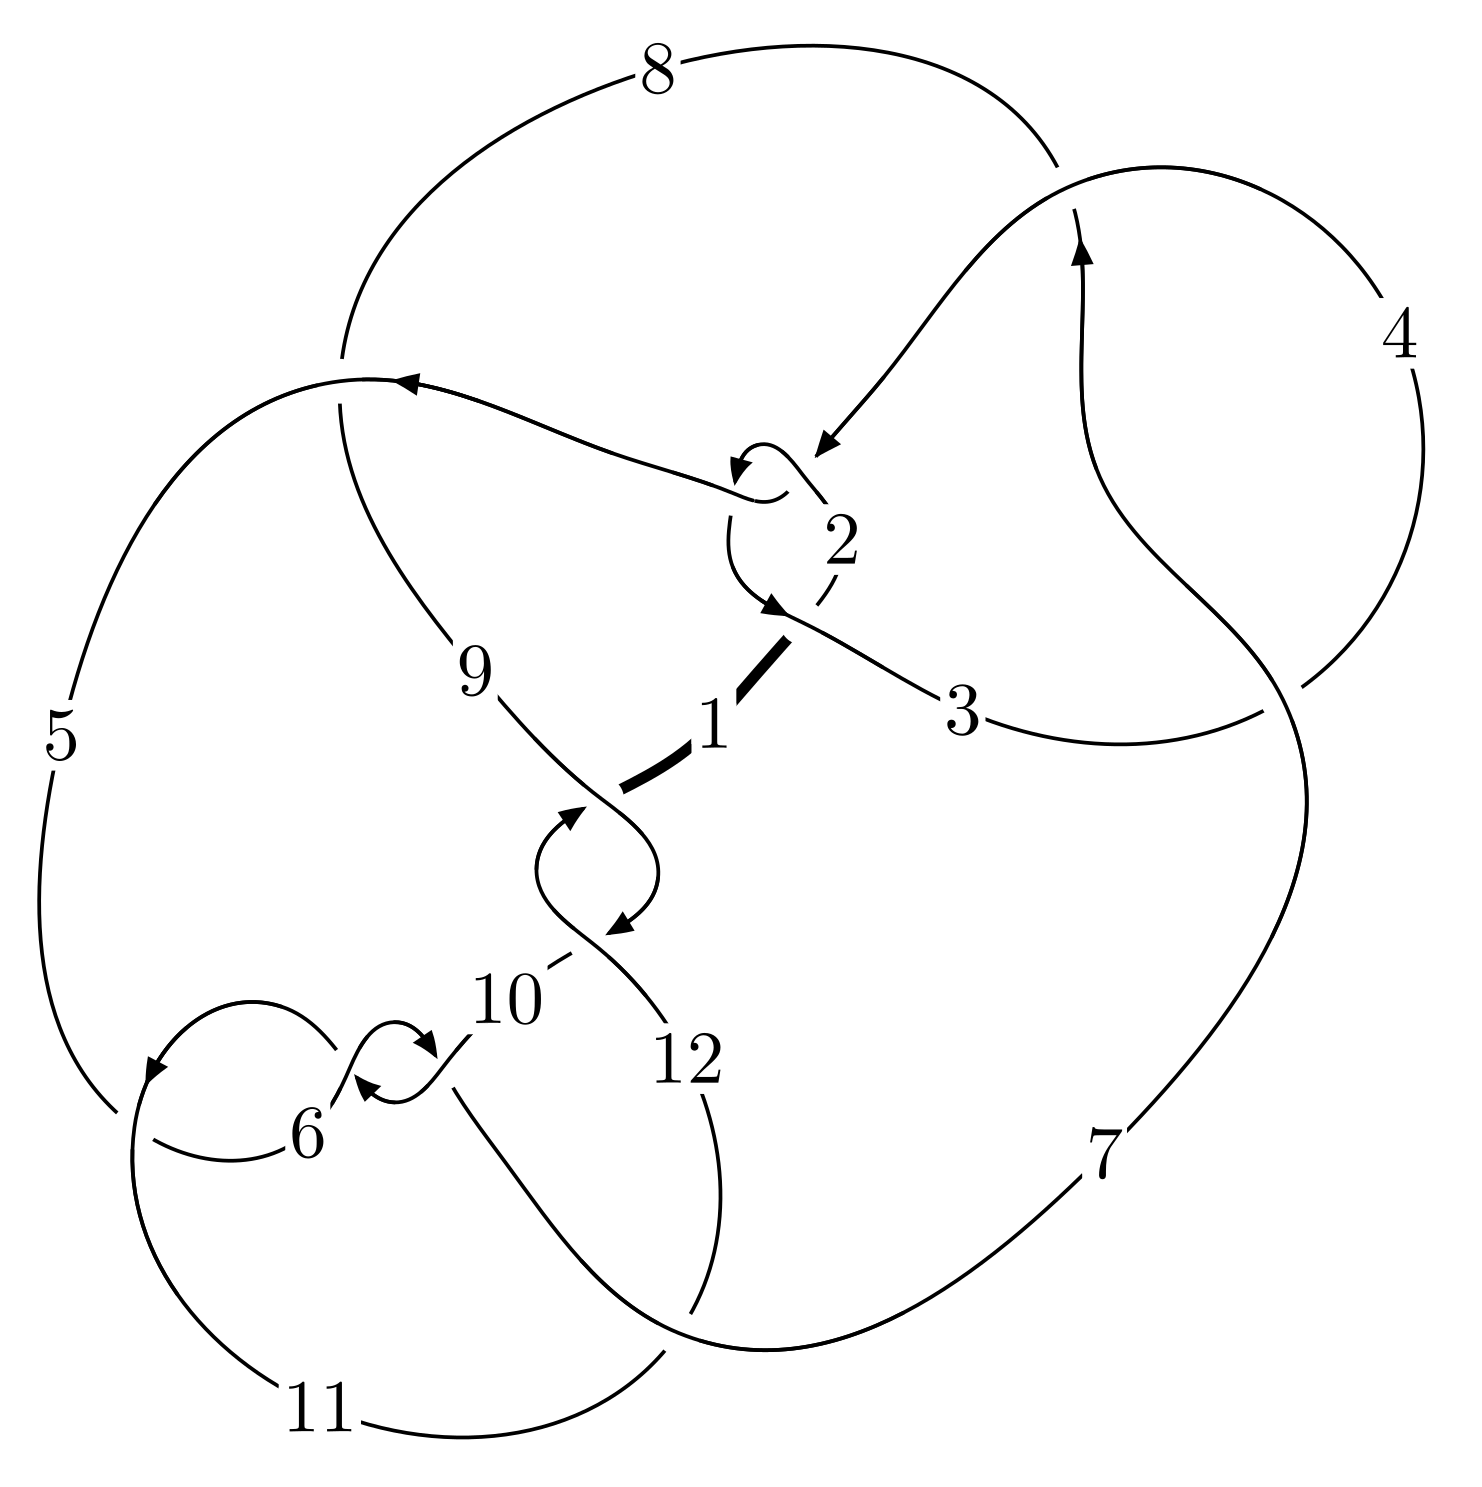
\includegraphics[width=112pt]{../../../GIT/diagram.site/Diagrams/png/2260_12n_0171.png}\\
\ \ \ A knot diagram\footnotemark}&
\allowdisplaybreaks
\textbf{Linearized knot diagam} \\
\cline{2-2}
 &
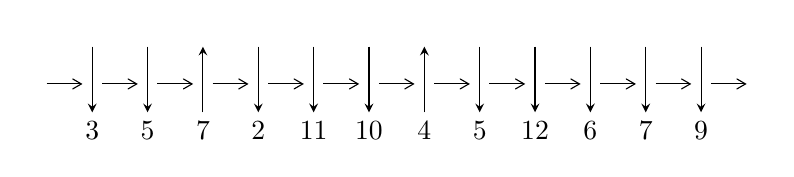
\begin{tikzpicture}[x=20pt, y=17pt]
	% nodes
	\node (C0) at (0, 0) {};
	\node (C1) at (1, 0) {};
	\node (C1U) at (1, +1) {};
	\node (C1D) at (1, -1) {3};

	\node (C2) at (2, 0) {};
	\node (C2U) at (2, +1) {};
	\node (C2D) at (2, -1) {5};

	\node (C3) at (3, 0) {};
	\node (C3U) at (3, +1) {};
	\node (C3D) at (3, -1) {7};

	\node (C4) at (4, 0) {};
	\node (C4U) at (4, +1) {};
	\node (C4D) at (4, -1) {2};

	\node (C5) at (5, 0) {};
	\node (C5U) at (5, +1) {};
	\node (C5D) at (5, -1) {11};

	\node (C6) at (6, 0) {};
	\node (C6U) at (6, +1) {};
	\node (C6D) at (6, -1) {10};

	\node (C7) at (7, 0) {};
	\node (C7U) at (7, +1) {};
	\node (C7D) at (7, -1) {4};

	\node (C8) at (8, 0) {};
	\node (C8U) at (8, +1) {};
	\node (C8D) at (8, -1) {5};

	\node (C9) at (9, 0) {};
	\node (C9U) at (9, +1) {};
	\node (C9D) at (9, -1) {12};

	\node (C10) at (10, 0) {};
	\node (C10U) at (10, +1) {};
	\node (C10D) at (10, -1) {6};

	\node (C11) at (11, 0) {};
	\node (C11U) at (11, +1) {};
	\node (C11D) at (11, -1) {7};

	\node (C12) at (12, 0) {};
	\node (C12U) at (12, +1) {};
	\node (C12D) at (12, -1) {9};
	\node (C13) at (13, 0) {};

	% arrows
	\draw[->,>={angle 60}]
	(C0) edge (C1) (C1) edge (C2) (C2) edge (C3) (C3) edge (C4) (C4) edge (C5) (C5) edge (C6) (C6) edge (C7) (C7) edge (C8) (C8) edge (C9) (C9) edge (C10) (C10) edge (C11) (C11) edge (C12) (C12) edge (C13) ;	\draw[->,>=stealth]
	(C1U) edge (C1D) (C2U) edge (C2D) (C3D) edge (C3U) (C4U) edge (C4D) (C5U) edge (C5D) (C6U) edge (C6D) (C7D) edge (C7U) (C8U) edge (C8D) (C9U) edge (C9D) (C10U) edge (C10D) (C11U) edge (C11D) (C12U) edge (C12D) ;
	\end{tikzpicture} \\
\hhline{~~} \\& 
\textbf{Solving Sequence} \\ \cline{2-2} 
 &
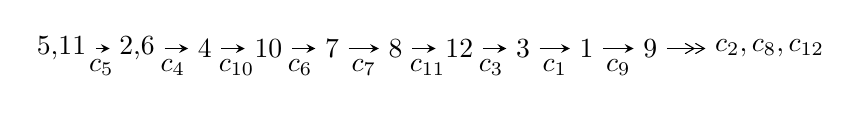
\begin{tikzpicture}[x=23pt, y=7pt]
	% node
	\node (A0) at (-1/8, 0) {5,11};
	\node (A1) at (17/16, 0) {2,6};
	\node (A2) at (17/8, 0) {4};
	\node (A3) at (25/8, 0) {10};
	\node (A4) at (33/8, 0) {7};
	\node (A5) at (41/8, 0) {8};
	\node (A6) at (49/8, 0) {12};
	\node (A7) at (57/8, 0) {3};
	\node (A8) at (65/8, 0) {1};
	\node (A9) at (73/8, 0) {9};
	\node (C1) at (1/2, -1) {$c_{5}$};
	\node (C2) at (13/8, -1) {$c_{4}$};
	\node (C3) at (21/8, -1) {$c_{10}$};
	\node (C4) at (29/8, -1) {$c_{6}$};
	\node (C5) at (37/8, -1) {$c_{7}$};
	\node (C6) at (45/8, -1) {$c_{11}$};
	\node (C7) at (53/8, -1) {$c_{3}$};
	\node (C8) at (61/8, -1) {$c_{1}$};
	\node (C9) at (69/8, -1) {$c_{9}$};
	\node (A10) at (11, 0) {$c_{2},c_{8},c_{12}$};

	% edge
	\draw[->,>=stealth]	
	(A0) edge (A1) (A1) edge (A2) (A2) edge (A3) (A3) edge (A4) (A4) edge (A5) (A5) edge (A6) (A6) edge (A7) (A7) edge (A8) (A8) edge (A9) ;
	\draw[->>,>={angle 60}]	
	(A9) edge (A10);
\end{tikzpicture} \\ 

\end{tabular} \\

\footnotetext{
The image of knot diagram is generated by the software ``\textbf{Draw programme}" developed by Andrew Bartholomew(\url{http://www.layer8.co.uk/maths/draw/index.htm\#Running-draw}), where we modified some parts for our purpose(\url{https://github.com/CATsTAILs/LinksPainter}).
}\phantom \\ \newline 
\centering \textbf{Ideals for irreducible components\footnotemark of $X_{\text{par}}$} 
 
\begin{align*}
I^u_{1}&=\langle 
- u^{23}+u^{22}+\cdots+6 u^2+b,\;- u^{21}+u^{20}+\cdots+a+2,\;u^{26}-2 u^{25}+\cdots+2 u-1\rangle \\
I^u_{2}&=\langle 
b+1,\;u^2+a+u+3,\;u^3+2 u-1\rangle \\
I^u_{3}&=\langle 
b+1,\;u^3+a+u+2,\;u^4+u^3+2 u^2+2 u+1\rangle \\
\\
\end{align*}
\raggedright * 3 irreducible components of $\dim_{\mathbb{C}}=0$, with total 33 representations.\\
\footnotetext{All coefficients of polynomials are rational numbers. But the coefficients are sometimes approximated in decimal forms when there is not enough margin.}
\newpage
\renewcommand{\arraystretch}{1}
\centering \section*{I. $I^u_{1}= \langle - u^{23}+u^{22}+\cdots+6 u^2+b,\;- u^{21}+u^{20}+\cdots+a+2,\;u^{26}-2 u^{25}+\cdots+2 u-1 \rangle$}
\flushleft \textbf{(i) Arc colorings}\\
\begin{tabular}{m{7pt} m{180pt} m{7pt} m{180pt} }
\flushright $a_{5}=$&$\begin{pmatrix}1\\0\end{pmatrix}$ \\
\flushright $a_{11}=$&$\begin{pmatrix}0\\u\end{pmatrix}$ \\
\flushright $a_{2}=$&$\begin{pmatrix}u^{21}- u^{20}+\cdots+6 u-2\\u^{23}- u^{22}+\cdots+12 u^3-6 u^2\end{pmatrix}$ \\
\flushright $a_{6}=$&$\begin{pmatrix}1\\u^2\end{pmatrix}$ \\
\flushright $a_{4}=$&$\begin{pmatrix}- u^{22}+u^{21}+\cdots+6 u-1\\- u^{22}+u^{21}+\cdots-6 u^2+u\end{pmatrix}$ \\
\flushright $a_{10}=$&$\begin{pmatrix}u\\u^3+u\end{pmatrix}$ \\
\flushright $a_{7}=$&$\begin{pmatrix}u^2+1\\u^4+2 u^2\end{pmatrix}$ \\
\flushright $a_{8}=$&$\begin{pmatrix}u^{11}+6 u^9+12 u^7+8 u^5+u^3+2 u\\u^{11}+5 u^9+8 u^7+3 u^5- u^3+u\end{pmatrix}$ \\
\flushright $a_{12}=$&$\begin{pmatrix}- u^5-2 u^3- u\\- u^7-3 u^5-2 u^3+u\end{pmatrix}$ \\
\flushright $a_{3}=$&$\begin{pmatrix}- u^{23}+u^{22}+\cdots+6 u-2\\u^{23}- u^{22}+\cdots+12 u^3-6 u^2\end{pmatrix}$ \\
\flushright $a_{1}=$&$\begin{pmatrix}u^{13}+6 u^{11}+13 u^9+12 u^7+6 u^5+4 u^3+u\\u^{15}+7 u^{13}+18 u^{11}+19 u^9+6 u^7+2 u^5+4 u^3- u\end{pmatrix}$ \\
\flushright $a_{9}=$&$\begin{pmatrix}u^9+4 u^7+5 u^5+2 u^3+u\\u^{11}+5 u^9+8 u^7+3 u^5- u^3+u\end{pmatrix}$\\&\end{tabular}
\flushleft \textbf{(ii) Obstruction class $= -1$}\\~\\
\flushleft \textbf{(iii) Cusp Shapes $= -4 u^{25}+8 u^{24}-59 u^{23}+102 u^{22}-370 u^{21}+552 u^{20}-1282 u^{19}+1632 u^{18}-2664 u^{17}+2824 u^{16}-3388 u^{15}+2869 u^{14}-2682 u^{13}+1765 u^{12}-1574 u^{11}+986 u^{10}-1012 u^9+713 u^8-547 u^7+276 u^6-182 u^5+78 u^4-102 u^3+80 u^2-8 u-13$}\\~\\
\newpage\renewcommand{\arraystretch}{1}
\flushleft \textbf{(iv) u-Polynomials at the component}\newline \\
\begin{tabular}{m{50pt}|m{274pt}}
Crossings & \hspace{64pt}u-Polynomials at each crossing \\
\hline $$\begin{aligned}c_{1}\end{aligned}$$&$\begin{aligned}
&u^{26}+30 u^{24}+\cdots+25 u+1
\end{aligned}$\\
\hline $$\begin{aligned}c_{2},c_{4}\end{aligned}$$&$\begin{aligned}
&u^{26}-8 u^{25}+\cdots+9 u-1
\end{aligned}$\\
\hline $$\begin{aligned}c_{3},c_{7}\end{aligned}$$&$\begin{aligned}
&u^{26}- u^{25}+\cdots-64 u+128
\end{aligned}$\\
\hline $$\begin{aligned}c_{5},c_{6},c_{10}\end{aligned}$$&$\begin{aligned}
&u^{26}+2 u^{25}+\cdots-2 u-1
\end{aligned}$\\
\hline $$\begin{aligned}c_{8}\end{aligned}$$&$\begin{aligned}
&u^{26}+2 u^{25}+\cdots+3088 u-11981
\end{aligned}$\\
\hline $$\begin{aligned}c_{9},c_{12}\end{aligned}$$&$\begin{aligned}
&u^{26}-2 u^{25}+\cdots-7 u^2+1
\end{aligned}$\\
\hline $$\begin{aligned}c_{11}\end{aligned}$$&$\begin{aligned}
&u^{26}-2 u^{25}+\cdots+48 u-72
\end{aligned}$\\
\hline
\end{tabular}\\~\\
\newpage\renewcommand{\arraystretch}{1}
\flushleft \textbf{(v) Riley Polynomials at the component}\newline \\
\begin{tabular}{m{50pt}|m{274pt}}
Crossings & \hspace{64pt}Riley Polynomials at each crossing \\
\hline $$\begin{aligned}c_{1}\end{aligned}$$&$\begin{aligned}
&y^{26}+60 y^{25}+\cdots-337 y+1
\end{aligned}$\\
\hline $$\begin{aligned}c_{2},c_{4}\end{aligned}$$&$\begin{aligned}
&y^{26}+30 y^{24}+\cdots-25 y+1
\end{aligned}$\\
\hline $$\begin{aligned}c_{3},c_{7}\end{aligned}$$&$\begin{aligned}
&y^{26}-45 y^{25}+\cdots-258048 y+16384
\end{aligned}$\\
\hline $$\begin{aligned}c_{5},c_{6},c_{10}\end{aligned}$$&$\begin{aligned}
&y^{26}+26 y^{25}+\cdots-14 y+1
\end{aligned}$\\
\hline $$\begin{aligned}c_{8}\end{aligned}$$&$\begin{aligned}
&y^{26}+122 y^{25}+\cdots-4243693030 y+143544361
\end{aligned}$\\
\hline $$\begin{aligned}c_{9},c_{12}\end{aligned}$$&$\begin{aligned}
&y^{26}+38 y^{25}+\cdots-14 y+1
\end{aligned}$\\
\hline $$\begin{aligned}c_{11}\end{aligned}$$&$\begin{aligned}
&y^{26}+18 y^{25}+\cdots-16272 y+5184
\end{aligned}$\\
\hline
\end{tabular}\\~\\
\newpage\flushleft \textbf{(vi) Complex Volumes and Cusp Shapes}
$$\begin{array}{c|c|c}  
\text{Solutions to }I^u_{1}& \I (\text{vol} + \sqrt{-1}CS) & \text{Cusp shape}\\
 \hline 
\begin{aligned}
u &= \phantom{-}0.703140 + 0.538371 I \\
a &= \phantom{-}0.595244 - 1.218420 I \\
b &= \phantom{-}1.13151 - 1.20043 I\end{aligned}
 & \phantom{-}14.5729 + 1.9359 I & -4.36941 + 0.69311 I \\ \hline\begin{aligned}
u &= \phantom{-}0.703140 - 0.538371 I \\
a &= \phantom{-}0.595244 + 1.218420 I \\
b &= \phantom{-}1.13151 + 1.20043 I\end{aligned}
 & \phantom{-}14.5729 - 1.9359 I & -4.36941 - 0.69311 I \\ \hline\begin{aligned}
u &= \phantom{-}0.729197 + 0.493462 I \\
a &= \phantom{-}2.28117 - 0.26467 I \\
b &= \phantom{-}1.17041 + 1.16109 I\end{aligned}
 & \phantom{-}14.4224 - 6.7123 I & -4.71846 + 4.71456 I \\ \hline\begin{aligned}
u &= \phantom{-}0.729197 - 0.493462 I \\
a &= \phantom{-}2.28117 + 0.26467 I \\
b &= \phantom{-}1.17041 - 1.16109 I\end{aligned}
 & \phantom{-}14.4224 + 6.7123 I & -4.71846 - 4.71456 I \\ \hline\begin{aligned}
u &= -0.657044 + 0.360115 I \\
a &= \phantom{-}1.94829 - 0.09632 I \\
b &= \phantom{-}0.522022 - 0.742639 I\end{aligned}
 & \phantom{-}3.09785 + 3.69296 I & -4.58596 - 5.59657 I \\ \hline\begin{aligned}
u &= -0.657044 - 0.360115 I \\
a &= \phantom{-}1.94829 + 0.09632 I \\
b &= \phantom{-}0.522022 + 0.742639 I\end{aligned}
 & \phantom{-}3.09785 - 3.69296 I & -4.58596 + 5.59657 I \\ \hline\begin{aligned}
u &= -0.532790 + 0.522258 I \\
a &= \phantom{-}0.281675 + 0.540170 I \\
b &= \phantom{-}0.345233 + 0.836005 I\end{aligned}
 & \phantom{-}3.71321 + 0.25250 I & -2.90666 - 1.69873 I \\ \hline\begin{aligned}
u &= -0.532790 - 0.522258 I \\
a &= \phantom{-}0.281675 - 0.540170 I \\
b &= \phantom{-}0.345233 - 0.836005 I\end{aligned}
 & \phantom{-}3.71321 - 0.25250 I & -2.90666 + 1.69873 I \\ \hline\begin{aligned}
u &= \phantom{-}0.146766 + 1.279190 I \\
a &= \phantom{-}1.289160 - 0.159208 I \\
b &= \phantom{-}0.339771 + 0.227061 I\end{aligned}
 & \phantom{-}2.95015 - 2.37770 I & -2.22960 + 4.04579 I \\ \hline\begin{aligned}
u &= \phantom{-}0.146766 - 1.279190 I \\
a &= \phantom{-}1.289160 + 0.159208 I \\
b &= \phantom{-}0.339771 - 0.227061 I\end{aligned}
 & \phantom{-}2.95015 + 2.37770 I & -2.22960 - 4.04579 I\\
 \hline 
 \end{array}$$\newpage$$\begin{array}{c|c|c}  
\text{Solutions to }I^u_{1}& \I (\text{vol} + \sqrt{-1}CS) & \text{Cusp shape}\\
 \hline 
\begin{aligned}
u &= -0.041859 + 1.351780 I \\
a &= -1.30338 - 1.15705 I \\
b &= -1.156640 + 0.215585 I\end{aligned}
 & \phantom{-}2.15651 + 1.07901 I & -3.64779 + 0.86156 I \\ \hline\begin{aligned}
u &= -0.041859 - 1.351780 I \\
a &= -1.30338 + 1.15705 I \\
b &= -1.156640 - 0.215585 I\end{aligned}
 & \phantom{-}2.15651 - 1.07901 I & -3.64779 - 0.86156 I \\ \hline\begin{aligned}
u &= \phantom{-}0.108685 + 1.405560 I \\
a &= \phantom{-}0.007384 + 1.006780 I \\
b &= -0.587676 - 0.621059 I\end{aligned}
 & \phantom{-}4.56460 - 2.76012 I & -2.16196 + 3.94765 I \\ \hline\begin{aligned}
u &= \phantom{-}0.108685 - 1.405560 I \\
a &= \phantom{-}0.007384 - 1.006780 I \\
b &= -0.587676 + 0.621059 I\end{aligned}
 & \phantom{-}4.56460 + 2.76012 I & -2.16196 - 3.94765 I \\ \hline\begin{aligned}
u &= -0.24567 + 1.43288 I \\
a &= \phantom{-}1.45979 + 0.68729 I \\
b &= \phantom{-}0.662222 - 0.763929 I\end{aligned}
 & \phantom{-}8.83594 + 6.98292 I & -1.16198 - 5.80218 I \\ \hline\begin{aligned}
u &= -0.24567 - 1.43288 I \\
a &= \phantom{-}1.45979 - 0.68729 I \\
b &= \phantom{-}0.662222 + 0.763929 I\end{aligned}
 & \phantom{-}8.83594 - 6.98292 I & -1.16198 + 5.80218 I \\ \hline\begin{aligned}
u &= \phantom{-}0.512846\phantom{ +0.000000I} \\
a &= \phantom{-}1.47619\phantom{ +0.000000I} \\
b &= \phantom{-}0.224405\phantom{ +0.000000I}\end{aligned}
 & -1.00355\phantom{ +0.000000I} & -9.54280\phantom{ +0.000000I} \\ \hline\begin{aligned}
u &= -0.17183 + 1.48536 I \\
a &= -0.125401 - 0.252038 I \\
b &= \phantom{-}0.312586 + 1.039960 I\end{aligned}
 & \phantom{-}10.21460 + 2.79653 I & \phantom{-0.000000 } 0. - 1.62269 I \\ \hline\begin{aligned}
u &= -0.17183 - 1.48536 I \\
a &= -0.125401 + 0.252038 I \\
b &= \phantom{-}0.312586 - 1.039960 I\end{aligned}
 & \phantom{-}10.21460 - 2.79653 I & \phantom{-0.000000 -}0. + 1.62269 I \\ \hline\begin{aligned}
u &= \phantom{-}0.25787 + 1.50930 I \\
a &= \phantom{-}1.32769 - 1.23506 I \\
b &= \phantom{-}1.21947 + 1.15279 I\end{aligned}
 & -18.5465 - 10.3199 I & -1.57367 + 4.71876 I\\
 \hline 
 \end{array}$$\newpage$$\begin{array}{c|c|c}  
\text{Solutions to }I^u_{1}& \I (\text{vol} + \sqrt{-1}CS) & \text{Cusp shape}\\
 \hline 
\begin{aligned}
u &= \phantom{-}0.25787 - 1.50930 I \\
a &= \phantom{-}1.32769 + 1.23506 I \\
b &= \phantom{-}1.21947 - 1.15279 I\end{aligned}
 & -18.5465 + 10.3199 I & -1.57367 - 4.71876 I \\ \hline\begin{aligned}
u &= \phantom{-}0.23540 + 1.52332 I \\
a &= -0.334114 - 0.224598 I \\
b &= \phantom{-}1.12696 - 1.25945 I\end{aligned}
 & -18.1670 - 1.4877 I & -1.145266 + 0.723281 I \\ \hline\begin{aligned}
u &= \phantom{-}0.23540 - 1.52332 I \\
a &= -0.334114 + 0.224598 I \\
b &= \phantom{-}1.12696 + 1.25945 I\end{aligned}
 & -18.1670 + 1.4877 I & -1.145266 - 0.723281 I \\ \hline\begin{aligned}
u &= \phantom{-}0.368033 + 0.267400 I \\
a &= -0.272224 + 1.261050 I \\
b &= -0.657600 - 0.268641 I\end{aligned}
 & -0.775564 - 1.043300 I & -8.38623 + 6.25558 I \\ \hline\begin{aligned}
u &= \phantom{-}0.368033 - 0.267400 I \\
a &= -0.272224 - 1.261050 I \\
b &= -0.657600 + 0.268641 I\end{aligned}
 & -0.775564 + 1.043300 I & -8.38623 - 6.25558 I \\ \hline\begin{aligned}
u &= -0.312651\phantom{ +0.000000I} \\
a &= -4.78676\phantom{ +0.000000I} \\
b &= -1.08095\phantom{ +0.000000I}\end{aligned}
 & -2.08164\phantom{ +0.000000I} & \phantom{-}2.25490\phantom{ +0.000000I}\\
 \hline 
 \end{array}$$\newpage\newpage\renewcommand{\arraystretch}{1}
\centering \section*{II. $I^u_{2}= \langle b+1,\;u^2+a+u+3,\;u^3+2 u-1 \rangle$}
\flushleft \textbf{(i) Arc colorings}\\
\begin{tabular}{m{7pt} m{180pt} m{7pt} m{180pt} }
\flushright $a_{5}=$&$\begin{pmatrix}1\\0\end{pmatrix}$ \\
\flushright $a_{11}=$&$\begin{pmatrix}0\\u\end{pmatrix}$ \\
\flushright $a_{2}=$&$\begin{pmatrix}- u^2- u-3\\-1\end{pmatrix}$ \\
\flushright $a_{6}=$&$\begin{pmatrix}1\\u^2\end{pmatrix}$ \\
\flushright $a_{4}=$&$\begin{pmatrix}- u^2- u-2\\-1\end{pmatrix}$ \\
\flushright $a_{10}=$&$\begin{pmatrix}u\\- u+1\end{pmatrix}$ \\
\flushright $a_{7}=$&$\begin{pmatrix}u^2+1\\u\end{pmatrix}$ \\
\flushright $a_{8}=$&$\begin{pmatrix}u^2+1\\u\end{pmatrix}$ \\
\flushright $a_{12}=$&$\begin{pmatrix}- u^2- u\\u^2\end{pmatrix}$ \\
\flushright $a_{3}=$&$\begin{pmatrix}- u^2- u-2\\-1\end{pmatrix}$ \\
\flushright $a_{1}=$&$\begin{pmatrix}-1\\0\end{pmatrix}$ \\
\flushright $a_{9}=$&$\begin{pmatrix}u^2- u+1\\u\end{pmatrix}$\\&\end{tabular}
\flushleft \textbf{(ii) Obstruction class $= 1$}\\~\\
\flushleft \textbf{(iii) Cusp Shapes $= -7 u^2-5 u-18$}\\~\\
\newpage\renewcommand{\arraystretch}{1}
\flushleft \textbf{(iv) u-Polynomials at the component}\newline \\
\begin{tabular}{m{50pt}|m{274pt}}
Crossings & \hspace{64pt}u-Polynomials at each crossing \\
\hline $$\begin{aligned}c_{1},c_{2}\end{aligned}$$&$\begin{aligned}
&(u-1)^3
\end{aligned}$\\
\hline $$\begin{aligned}c_{3},c_{7}\end{aligned}$$&$\begin{aligned}
&u^3
\end{aligned}$\\
\hline $$\begin{aligned}c_{4}\end{aligned}$$&$\begin{aligned}
&(u+1)^3
\end{aligned}$\\
\hline $$\begin{aligned}c_{5},c_{6},c_{9}\end{aligned}$$&$\begin{aligned}
&u^3+2 u-1
\end{aligned}$\\
\hline $$\begin{aligned}c_{8},c_{10},c_{12}\end{aligned}$$&$\begin{aligned}
&u^3+2 u+1
\end{aligned}$\\
\hline $$\begin{aligned}c_{11}\end{aligned}$$&$\begin{aligned}
&u^3+3 u^2+5 u+2
\end{aligned}$\\
\hline
\end{tabular}\\~\\
\newpage\renewcommand{\arraystretch}{1}
\flushleft \textbf{(v) Riley Polynomials at the component}\newline \\
\begin{tabular}{m{50pt}|m{274pt}}
Crossings & \hspace{64pt}Riley Polynomials at each crossing \\
\hline $$\begin{aligned}c_{1},c_{2},c_{4}\end{aligned}$$&$\begin{aligned}
&(y-1)^3
\end{aligned}$\\
\hline $$\begin{aligned}c_{3},c_{7}\end{aligned}$$&$\begin{aligned}
&y^3
\end{aligned}$\\
\hline $$\begin{aligned}c_{5},c_{6},c_{8}\\c_{9},c_{10},c_{12}\end{aligned}$$&$\begin{aligned}
&y^3+4 y^2+4 y-1
\end{aligned}$\\
\hline $$\begin{aligned}c_{11}\end{aligned}$$&$\begin{aligned}
&y^3+y^2+13 y-4
\end{aligned}$\\
\hline
\end{tabular}\\~\\
\newpage\flushleft \textbf{(vi) Complex Volumes and Cusp Shapes}
$$\begin{array}{c|c|c}  
\text{Solutions to }I^u_{2}& \I (\text{vol} + \sqrt{-1}CS) & \text{Cusp shape}\\
 \hline 
\begin{aligned}
u &= -0.22670 + 1.46771 I \\
a &= -0.670516 - 0.802255 I \\
b &= -1.00000\phantom{ +0.000000I}\end{aligned}
 & \phantom{-}7.79580 + 5.13794 I & -2.14701 - 2.68036 I \\ \hline\begin{aligned}
u &= -0.22670 - 1.46771 I \\
a &= -0.670516 + 0.802255 I \\
b &= -1.00000\phantom{ +0.000000I}\end{aligned}
 & \phantom{-}7.79580 - 5.13794 I & -2.14701 + 2.68036 I \\ \hline\begin{aligned}
u &= \phantom{-}0.453398\phantom{ +0.000000I} \\
a &= -3.65897\phantom{ +0.000000I} \\
b &= -1.00000\phantom{ +0.000000I}\end{aligned}
 & -2.43213\phantom{ +0.000000I} & -21.7060\phantom{ +0.000000I}\\
 \hline 
 \end{array}$$\newpage\newpage\renewcommand{\arraystretch}{1}
\centering \section*{III. $I^u_{3}= \langle b+1,\;u^3+a+u+2,\;u^4+u^3+2 u^2+2 u+1 \rangle$}
\flushleft \textbf{(i) Arc colorings}\\
\begin{tabular}{m{7pt} m{180pt} m{7pt} m{180pt} }
\flushright $a_{5}=$&$\begin{pmatrix}1\\0\end{pmatrix}$ \\
\flushright $a_{11}=$&$\begin{pmatrix}0\\u\end{pmatrix}$ \\
\flushright $a_{2}=$&$\begin{pmatrix}- u^3- u-2\\-1\end{pmatrix}$ \\
\flushright $a_{6}=$&$\begin{pmatrix}1\\u^2\end{pmatrix}$ \\
\flushright $a_{4}=$&$\begin{pmatrix}- u^3- u-1\\-1\end{pmatrix}$ \\
\flushright $a_{10}=$&$\begin{pmatrix}u\\u^3+u\end{pmatrix}$ \\
\flushright $a_{7}=$&$\begin{pmatrix}u^2+1\\- u^3-2 u-1\end{pmatrix}$ \\
\flushright $a_{8}=$&$\begin{pmatrix}u^2+1\\- u^3-2 u-1\end{pmatrix}$ \\
\flushright $a_{12}=$&$\begin{pmatrix}- u^3-2 u-1\\- u^3- u^2- u-2\end{pmatrix}$ \\
\flushright $a_{3}=$&$\begin{pmatrix}- u^3- u-1\\-1\end{pmatrix}$ \\
\flushright $a_{1}=$&$\begin{pmatrix}-1\\0\end{pmatrix}$ \\
\flushright $a_{9}=$&$\begin{pmatrix}u^3+u^2+2 u+2\\- u^3-2 u-1\end{pmatrix}$\\&\end{tabular}
\flushleft \textbf{(ii) Obstruction class $= 1$}\\~\\
\flushleft \textbf{(iii) Cusp Shapes $= -3 u^3+2 u^2-2 u-7$}\\~\\
\newpage\renewcommand{\arraystretch}{1}
\flushleft \textbf{(iv) u-Polynomials at the component}\newline \\
\begin{tabular}{m{50pt}|m{274pt}}
Crossings & \hspace{64pt}u-Polynomials at each crossing \\
\hline $$\begin{aligned}c_{1},c_{2}\end{aligned}$$&$\begin{aligned}
&(u-1)^4
\end{aligned}$\\
\hline $$\begin{aligned}c_{3},c_{7}\end{aligned}$$&$\begin{aligned}
&u^4
\end{aligned}$\\
\hline $$\begin{aligned}c_{4}\end{aligned}$$&$\begin{aligned}
&(u+1)^4
\end{aligned}$\\
\hline $$\begin{aligned}c_{5},c_{6},c_{9}\end{aligned}$$&$\begin{aligned}
&u^4+u^3+2 u^2+2 u+1
\end{aligned}$\\
\hline $$\begin{aligned}c_{8},c_{10},c_{12}\end{aligned}$$&$\begin{aligned}
&u^4- u^3+2 u^2-2 u+1
\end{aligned}$\\
\hline $$\begin{aligned}c_{11}\end{aligned}$$&$\begin{aligned}
&(u^2- u+1)^2
\end{aligned}$\\
\hline
\end{tabular}\\~\\
\newpage\renewcommand{\arraystretch}{1}
\flushleft \textbf{(v) Riley Polynomials at the component}\newline \\
\begin{tabular}{m{50pt}|m{274pt}}
Crossings & \hspace{64pt}Riley Polynomials at each crossing \\
\hline $$\begin{aligned}c_{1},c_{2},c_{4}\end{aligned}$$&$\begin{aligned}
&(y-1)^4
\end{aligned}$\\
\hline $$\begin{aligned}c_{3},c_{7}\end{aligned}$$&$\begin{aligned}
&y^4
\end{aligned}$\\
\hline $$\begin{aligned}c_{5},c_{6},c_{8}\\c_{9},c_{10},c_{12}\end{aligned}$$&$\begin{aligned}
&y^4+3 y^3+2 y^2+1
\end{aligned}$\\
\hline $$\begin{aligned}c_{11}\end{aligned}$$&$\begin{aligned}
&(y^2+y+1)^2
\end{aligned}$\\
\hline
\end{tabular}\\~\\
\newpage\flushleft \textbf{(vi) Complex Volumes and Cusp Shapes}
$$\begin{array}{c|c|c}  
\text{Solutions to }I^u_{3}& \I (\text{vol} + \sqrt{-1}CS) & \text{Cusp shape}\\
 \hline 
\begin{aligned}
u &= -0.621744 + 0.440597 I \\
a &= -1.50000 - 0.86603 I \\
b &= -1.00000\phantom{ +0.000000I}\end{aligned}
 & \phantom{-}1.64493 + 2.02988 I & -5.73686 - 3.25323 I \\ \hline\begin{aligned}
u &= -0.621744 - 0.440597 I \\
a &= -1.50000 + 0.86603 I \\
b &= -1.00000\phantom{ +0.000000I}\end{aligned}
 & \phantom{-}1.64493 - 2.02988 I & -5.73686 + 3.25323 I \\ \hline\begin{aligned}
u &= \phantom{-}0.121744 + 1.306620 I \\
a &= -1.50000 + 0.86603 I \\
b &= -1.00000\phantom{ +0.000000I}\end{aligned}
 & \phantom{-}1.64493 - 2.02988 I & -8.76314 + 4.54099 I \\ \hline\begin{aligned}
u &= \phantom{-}0.121744 - 1.306620 I \\
a &= -1.50000 - 0.86603 I \\
b &= -1.00000\phantom{ +0.000000I}\end{aligned}
 & \phantom{-}1.64493 + 2.02988 I & -8.76314 - 4.54099 I\\
 \hline 
 \end{array}$$\newpage
\newpage\renewcommand{\arraystretch}{1}
\centering \section*{ IV. u-Polynomials}
\begin{tabular}{m{50pt}|m{274pt}}
Crossings & \hspace{64pt}u-Polynomials at each crossing \\
\hline $$\begin{aligned}c_{1}\end{aligned}$$&$\begin{aligned}
&((u-1)^7)(u^{26}+30 u^{24}+\cdots+25 u+1)
\end{aligned}$\\
\hline $$\begin{aligned}c_{2}\end{aligned}$$&$\begin{aligned}
&((u-1)^7)(u^{26}-8 u^{25}+\cdots+9 u-1)
\end{aligned}$\\
\hline $$\begin{aligned}c_{3},c_{7}\end{aligned}$$&$\begin{aligned}
&u^7(u^{26}- u^{25}+\cdots-64 u+128)
\end{aligned}$\\
\hline $$\begin{aligned}c_{4}\end{aligned}$$&$\begin{aligned}
&((u+1)^7)(u^{26}-8 u^{25}+\cdots+9 u-1)
\end{aligned}$\\
\hline $$\begin{aligned}c_{5},c_{6}\end{aligned}$$&$\begin{aligned}
&(u^3+2 u-1)(u^4+u^3+2 u^2+2 u+1)(u^{26}+2 u^{25}+\cdots-2 u-1)
\end{aligned}$\\
\hline $$\begin{aligned}c_{8}\end{aligned}$$&$\begin{aligned}
&(u^3+2 u+1)(u^4- u^3+2 u^2-2 u+1)(u^{26}+2 u^{25}+\cdots+3088 u-11981)
\end{aligned}$\\
\hline $$\begin{aligned}c_{9}\end{aligned}$$&$\begin{aligned}
&(u^3+2 u-1)(u^4+u^3+2 u^2+2 u+1)(u^{26}-2 u^{25}+\cdots-7 u^2+1)
\end{aligned}$\\
\hline $$\begin{aligned}c_{10}\end{aligned}$$&$\begin{aligned}
&(u^3+2 u+1)(u^4- u^3+2 u^2-2 u+1)(u^{26}+2 u^{25}+\cdots-2 u-1)
\end{aligned}$\\
\hline $$\begin{aligned}c_{11}\end{aligned}$$&$\begin{aligned}
&((u^2- u+1)^2)(u^3+3 u^2+5 u+2)(u^{26}-2 u^{25}+\cdots+48 u-72)
\end{aligned}$\\
\hline $$\begin{aligned}c_{12}\end{aligned}$$&$\begin{aligned}
&(u^3+2 u+1)(u^4- u^3+2 u^2-2 u+1)(u^{26}-2 u^{25}+\cdots-7 u^2+1)
\end{aligned}$\\
\hline
\end{tabular}\newpage\renewcommand{\arraystretch}{1}
\centering \section*{ V. Riley Polynomials}
\begin{tabular}{m{50pt}|m{274pt}}
Crossings & \hspace{64pt}Riley Polynomials at each crossing \\
\hline $$\begin{aligned}c_{1}\end{aligned}$$&$\begin{aligned}
&((y-1)^7)(y^{26}+60 y^{25}+\cdots-337 y+1)
\end{aligned}$\\
\hline $$\begin{aligned}c_{2},c_{4}\end{aligned}$$&$\begin{aligned}
&((y-1)^7)(y^{26}+30 y^{24}+\cdots-25 y+1)
\end{aligned}$\\
\hline $$\begin{aligned}c_{3},c_{7}\end{aligned}$$&$\begin{aligned}
&y^7(y^{26}-45 y^{25}+\cdots-258048 y+16384)
\end{aligned}$\\
\hline $$\begin{aligned}c_{5},c_{6},c_{10}\end{aligned}$$&$\begin{aligned}
&(y^3+4 y^2+4 y-1)(y^4+3 y^3+2 y^2+1)(y^{26}+26 y^{25}+\cdots-14 y+1)
\end{aligned}$\\
\hline $$\begin{aligned}c_{8}\end{aligned}$$&$\begin{aligned}
&(y^3+4 y^2+4 y-1)(y^4+3 y^3+2 y^2+1)\\
&\cdot(y^{26}+122 y^{25}+\cdots-4243693030 y+143544361)
\end{aligned}$\\
\hline $$\begin{aligned}c_{9},c_{12}\end{aligned}$$&$\begin{aligned}
&(y^3+4 y^2+4 y-1)(y^4+3 y^3+2 y^2+1)(y^{26}+38 y^{25}+\cdots-14 y+1)
\end{aligned}$\\
\hline $$\begin{aligned}c_{11}\end{aligned}$$&$\begin{aligned}
&((y^2+y+1)^2)(y^3+y^2+13 y-4)(y^{26}+18 y^{25}+\cdots-16272 y+5184)
\end{aligned}$\\
\hline
\end{tabular}
\vskip 2pc
\end{document}